\documentclass{article}

\usepackage{arxiv}

\usepackage[utf8]{inputenc} % allow utf-8 input
\usepackage[T1]{fontenc}    % use 8-bit T1 fonts
\usepackage{hyperref}       % hyperlinks
\usepackage{url}            % simple URL typesetting
\usepackage{booktabs}       % professional-quality tables
\usepackage{amsfonts}       % blackboard math symbols
\usepackage{amsmath}
\usepackage{nicefrac}       % compact symbols for 1/2, etc.
\usepackage{microtype}      % microtypography
\usepackage{cleveref}       % smart cross-referencing
\usepackage{lipsum}         % Can be removed after putting your text content
\usepackage{graphicx}
\usepackage{natbib}
\usepackage{doi}

\title{A Motion Capture and Imitation Learning-based Approach to Robot Control}

% Here you can change the date presented in the paper title
%\date{September 9, 1985}
% Or remove it
%\date{}

\author{ \href{https://orcid.org/0000-0002-8956-179X}{
\includegraphics[scale=0.06]{orcid.pdf}\hspace{1mm}Peteris Racinskis}\thanks{Robotics and Machine Perception Laboratory} \thanks{Institute of Electronics and Computer Science, Riga, Latvia} \\
	\texttt{peteris.racinskis@edi.lv} \\
	%% examples of more authors
	\And
	\href{https://orcid.org/0000-0001-5203-3347}{
\includegraphics[scale=0.06]{orcid.pdf}\hspace{1mm}Janis Arents}\footnote[1]{test} \footnote[2]{test}\\
	\texttt{janis.arents@edi.lv} \\
	\And
	\href{https://orcid.org/0000-0002-5405-0738}{
\includegraphics[scale=0.06]{orcid.pdf}\hspace{1mm}Modris Greitans}\footnote[2]{} \\
	\texttt{modris\_greitans@edi.lv} \\
}

% Uncomment to override  the `A preprint' in the header
%\renewcommand{\headeright}{Technical Report}
%\renewcommand{\undertitle}{Technical Report}
\renewcommand{\shorttitle}{Motion Capture and Imitation Learning-based Robot Control}

%%% Add PDF metadata to help others organize their library
%%% Once the PDF is generated, you can check the metadata with
%%% $ pdfinfo template.pdf
\hypersetup{
pdftitle={A Motion Capture and Imitation Learning-Based Approach to Robot Control},
pdfsubject={cs.RO},
pdfauthor={Peteris Racinskis, Janis Arents, Modris Greitans},
pdfkeywords={Imitation Learning, Motion capture, Robotics, Artificial neural networks, RNN},
}

\begin{document}
\maketitle

\begin{abstract}
	Imitation Learning is a discipline of Machine Learning primarily concerned with replicating observed behavior of agents known to perform well on a given task, collected in demonstration data sets. In an industrial robotics context this presents the opportunity to replace explicit programming of behavior with demonstrations of the task to be performed. Motion capture is one of the methods for recording such data. It enables lesser model complexity compared to more indirect observation modalities such as visual data, yet requires additional data pre-processing if signals beyond a time series of effector positions and orientations are relevant to the task at hand. In this paper, an approach for motion capture-based imitation learning and implicit control signal estimation is introduced and evaluated on an object throwing task.
\end{abstract}


% keywords can be removed
\keywords{Imitation Learning \and Motion capture \and Robotics \and Artificial neural networks \and RNN}


\section{Introduction}

Manipulator arms and other types of robots have become ubiquitous in modern industry and their use has been proliferating for decades, yet even now the primary method for programming these devices remains procedural code, hand-crafted by specially trained technicians and engineers. This significantly increases the cost and complexity of commissioning process nodes that utilize industrial robots. To this end, various alternative approaches grounded in machine learning have been proposed. Perhaps the most commonly studied are methods that fall under the umbrella of reinforcement learning, which optimize an agent acting on its environment through the use of an explicitly specified reward function \citep{sutton2018reinforcement}. While offering strong theoretical guarantees of convergence, they require interaction with the environment for learning to occur. Furthermore, in practical settings the reward function for many tasks is very sparse, leading to large search spaces and inefficient exploration \citep{hester2018deep}. Finally, the reward function for a task may be unknown or difficult to specify analytically \citep{abbeel2004apprenticeship}.

Imitation learning is a broad field of study in its own right that promises to overcome some or all of the aforementioned challenges, provided that it is possible to obtain a corpus of demonstrations showing how the task is to be accomplished. When dealing with industrial robotics, this is often the case as the tasks we wish to execute are ones that human operators already routinely perform. Therefore, we have developed an approach for recording actions taken by humans in the physical environment, programmatically producing a training data set structured in the form of explicit demonstrations augmented with additional, extrapolated state inputs and control signals, and training artificial neural network models to reproduce the trajectories therein as motion plans.

Given the inherent trade-off between task specificity and required model complexity when it comes to observation data modality and model output, motion capture has been selected as a convenient middle ground. It does not require a simulated environment as approaches that involve virtual reality do \citep{zhang2018deep,dyrstad2018teaching}, obviates any issues that may come with having to learn motions in robot configuration space by operating in Cartesian coordinates, and does not necessitate the use of complex image processing layers as found in models with visual input modalities \citep{liu2018imitation, zhang2018deep}. The main drawbacks of this approach are that it requires motion capture equipment, which is more expensive than conventional video cameras, and Cartesian motion plans need an additional conversion step into joint space trajectories before it is possible to execute them on a real robot. Given the intended application of this system -- programming robots to perform tasks in an industrial environment -- the advantages of compact models, rapid training times and results that are possible to evaluate ahead of time were deemed to outweigh the drawbacks.

To help guide the development process and serve as a means of evaluation, a sample use case was selected -- object throwing with the goal of extending the robot's reach and improving cycle times. In particular, the task of robotically sorting plastic bottles at a recycling plant was to be augmented with a throwing capability. While on the surface the task is almost entirely defined by elementary ballistics that can be programmed explicitly, it serves as a convenient benchmark for robot programming by way of demonstrations. The task was deemed sufficiently non-trivial when considered from the perspective of a Markov decision process or time-series model only given limited information about system state at any given time step, while also being suitable for intuitive evaluation by human observers due to its intuitively straightforward nature. Furthermore, the relationship between release position, velocity and target coordinates provides an obvious way to quantitatively evaluate model performance against training and validation data -- extrapolated throw accuracy.


\section{Preliminaries}
\label{sec:prelim}

In this article, an \emph{agent} can be taken to mean the part of the system that acts based on state or observation information $s$ in an \emph{environment}, according to a \emph{policy} $\pi$ which is specified by a parametric \emph{model} -- a function $\pi_{\theta}(s)$ with parameters $\theta$ tuned in optimization and produces an output \emph{action} $a$. In practice this means that references to the agent, model and policy are almost interchangeable in most contexts. A formalism common in both reinforcement and imitation learning contexts is the \emph{Markov decision process} (MDP), formally given by \citep{attia2018global}

\begin{equation}
	MDP = (S,A,T,R,I)
\end{equation}
where $S$ is the set of states $s$, $A$ is the (formally discrete) set of actions $a$, $T:S \times A \rightarrow S$ is a state transition function that encapsulates the environment, $R:S \rightarrow \mathbb{R}$ is a reward function associated with each state and $I = p\left(s_0 \in S\right)$ represents the initial state distribution. In many imitation learning-related cases a reward function need not specified or considered. Moreover, if one is willing to break with the strict formal definition and give up the use of mathematical tools defined only on finite probability distributions, continuous action spaces can also be considered.

One important characteristic of the MDP is that it is history-agnostic -- the future state distribution of the system is uniquely defined by its current state. While technically true for physical environments, it is often the case that instead of a complete state representation vector $\mathbf{s}$ we are instead operating on a more limited \emph{observation} $\mathbf{o}$ (often interchangeably referred to as $\mathbf{s}$ for brevity), where each element $o_i$ is given by some function $f_i(\mathbf{s})$. It is therefore possible that historical observations contain information about hidden system state variables even assuming the MDP formalism holds for the underlying environment. An example of this can be the case when individual observations contain only the current position of an object but not its derivatives, as in video data. In such situations it may prove beneficial to break with the formalism further, by redefining the policy to operate on sequences of $k+1$ previous states/observations

\begin{equation}
	t, k, n \in \mathbb{N}, \pi_{\theta}:\lbrace {(s_n)_{t-k}^t} \rbrace \rightarrow A
\end{equation}
which, by allowing for input sequences of variable length, may become a function defined on the entire known state history:

\begin{equation}
	\pi_{\theta}:\lbrace {(s_n)_1^t} \rbrace \rightarrow A
\end{equation}

These adjustments allow for the employment of sequence-to-sequence predictor architectures also studied in other areas of machine learning such as recurrent neural networks (RNNs) \citep{rumelhart1985learning} and transformers \citep{vaswani2017attention}. Finally, if continuous action spaces are permitted it is no great stretch to also consider formats where the action corresponds to a predicted future state to be used for static motion planning or in a feedback controller

\begin{equation}
	\pi_{\theta}:\lbrace {(s_n)_1^t} \rbrace \rightarrow S
\end{equation}
which, when running the model on its own output, is equivalent to sequence building tasks encountered in domains such as text generation. 


\section{Related Work}
\label{sec:related}

In its simplest and most straightforward form -- sometimes referred to as \emph{behavioral cloning} -- imitation learning can be reduced to a classification or regression task. Given a set of states and actions or state transitions produced by an unknown expert function, a model (\emph{policy}) is trained to approximate this function. Even with very small parameter counts by modern standards, when combined with artificial neural networks this method has demonstrated some success as far back as the 1980s, provided a task with simple dynamics such as keeping a motor vehicle centered on a road \citep{pomerleau1989alvinn}.

However, it has since become apparent that pure behavioral cloning suffers from distribution shift -- a phenomenon whereby the distribution of states visited by the policy diverges from that of the original training data set by way of incremental error, eventually leading to poor predictions by the model and irrecoverable deviation from the intended task. To improve the ability of policies to recover from this failure mode, various more complex approaches to the task have been proposed. One major direction of research has been the use of inherently robust, composable functions known as \emph{dynamic motion primitives}, employing systems of differential equations and parametric models such as Gaussian basis functions to obviate the problem of distribution shift entirely -- ensuring convergence towards the goal through the explicit dynamics of the system \citep{pastor2009learning}. Though showing promising results, it must be noted that the model templates used are quite domain-specific. Others have attempted to use more general-purpose models in conjunction with interactive sampling of the expert response to compensate for distribution shift \citep{ross2011no}. While theoretically able to guarantee convergence, the major drawback of such methods is that an expert function is required that can be queried numerous times as part of the training process. This severely restricts applicability to practical use cases, since it is impossible to implement when only given a set of pre-recorded demonstrations.

A different means of handling this problem is given by the field of \emph{inverse reinforcement learning} \citep{abbeel2004apprenticeship}. Rather than attempting to model the expert function directly, it is assumed that the expert is itself acting in accordance with an unknown reward function. An attempt therefore is made to approximate this reward in a way that explains the observed behavior. From there this becomes a classical reinforcement learning problem, and any training method or model architecture developed in the space of this adjacent field of study can be employed. Where early approaches made certain assumptions about the form of this reward function -- such as it being linear -- more recent work has proposed that generative adversarial networks be used where the discriminator can approximate the class of all possible reward functions fitting the observations over an iterative training process \citep{ho2016generative}.

Perhaps the most promising results, however, come from the sequence modelling domain. Recurrent neural networks show up in earlier scientific literature periodically, such as in predicting a time-series of robot end effector loads in an assembly task \citep{scherzinger2019contact} and learning latent action plans from large, uncategorized play data sets \citep{lynch2020learning}. But current state-of-the-art performance across a wide variety of sequence prediction tasks -- among them imitation learning in a robotics context -- is given by combining a large, universal transformer model with embedding schemes specific to various data modalities \citep{reed2022generalist}. These results strongly suggest that structuring one's approach to be compatible with general-purpose sequence predictor algorithms is preferable for ensuring its longevity.

When it comes to the use of motion capture data, previous work in the robotics and imitation learning corner is quite sparse, possibly due to the costly and specialized nature of the equipment involved. One previously considered direction has been the use of consumer-grade motion tracking equipment for collecting demonstrations \citep{jha2017imitation}. Unlike our work, they employ a single, relatively inexpensive sensor unit to generate the motion tracking data, and the main focus of the work is on accurate extraction of the demonstrations rather than modelling and extrapolation -- which is left as something of an afterthought, with cluster and k-nearest interpolation methods used for inference. Outside the imitation learning space, related work has been done in human motion modelling utilizing RNNs trained on motion capture data \citep{Fragkiadaki_2015_ICCV}. The main difference between research in this direction and our work lies in the fact that we are looking for ways to translate human motion into paths taken by a robot, and do not consider the human kinematic model. Additionally, we place an emphasis on extracting particular implicit signals such as release timing and desired target coordinates. 

Meanwhile, optimal execution of object throwing tasks has been previously studied in a reinforcement learning context, such as with \emph{TossingBot} \citep{zeng2020tossingbot}. Their approach is radically different from ours, in that it utilizes a reinforcement learning policy to predict a set of grasp and throw parameters. These serve as inputs for grasping and throwing motion primitives. The throwing primitive itself is not learned, but provided with a release position and velocity, which it then executes. Initial estimates are produced analytically, which are then combined with learned residuals. The main distinction between their work and ours, however, is that of purpose. We do not seek to perfect an approach to throwing in particular, but rather establish a method for using imitation learning to program industrial robots. There is an expectation of being able to further adapt them for a variety of tasks -- with throwing serving primarily as a convenient benchmark for progress.

\section{Proposed approach}
\label{sec:approach}

Three crucial decisions need to be made when devising an imitation learning-based approach to robot control:
\begin{itemize}
	\item Data collection -- what will serve as the expert policy? How will data be obtained?
	\item Model architecture -- what type of model template will be used to learn the policy? What are its inputs and outputs, what pre- and post-processing steps will these formats call for?
	\item Control method -- how will model outputs be used in robot motion planning or feedback control?
\end{itemize}

Considering that the goal of this paper is not to examine any of these sub-problems in detail but rather to come up with a holistic approach to combine all of them, trade-offs that affect more than one step at a time need to be considered. Recording of human performances as the expert data set is also a constraint imposed by the objective we set out to accomplish. Therefore, when selecting the demonstration data modality, three possibilities were examined:
\begin{itemize}
	\item raw video -- using conventional cameras to record a scene and use these observations as model inputs directly;
	\item motion capture -- obtain effector and scene object pose (position and orientation) data with specialized motion capture equipment that consists of multiple cameras tracking highly reflective markers affixed to bodies of interest;
	\item simulation -- using a simulated environment in conjunction with virtual reality (VR) or other human-machine interface to obtain either pose data as with motion capture, or record the configurations of a robot model directly. 
\end{itemize}

Raw video is the most attractive approach from a material standpoint -- it does not involve motion capture or VR equipment, does not require simulated environments, and in principle presents the possibility of a sensor-to-actuator learned pipeline, if the video data were used directly in the model's input to predict joint velocities. In practice, however, not only does using image data call for the employment of more complex model architectures such as convolutional neural networks, images are inherently 2-dimensional representations of 3-dimensional space, leading to ambiguities in the data -- and one quickly runs into difficult issues such as context translation that confound the issue further \citep{liu2018imitation}. 

In contrast, unambiguous pose information is readily obtained with motion capture or simulation. Simulating a robot and collecting data in joint space allows for a simple final controller stage. But it very tightly couples the trained model to a specific physical implementation, and reasoning about or debugging model outputs obtained this way is not straightforward. Thus, the main comparison is to be drawn between object pose data as obtained in a simulation and with motion capture. Assuming motion capture equipment is available, setting the scene up for collecting demonstrations is a matter of outfitting the objects of interest with markers and defining them as rigid bodies to be tracked. However, there is a degree of imprecision in the observations, and information about different rigid bodies is available at different instants in time. 

Simulation allows recording exact pose information directly at regular time intervals, but setting up the scene necessitates creating a virtual environment where the task can be performed. In addition, for realistic interactions a physics simulation and immersive interface such as VR is required, but even this does not present the human demonstrator with the haptic feedback of actually performing the task in the real world. As such we decided that the benefits of simple setup and inherently natural interaction with the physical scene outweigh the precision and cost advantages of simulated environments, and selected motion capture as the source of demonstration data. For extracting additional information specific to the throwing task, we also track the object thrown and use its pose information to annotate each observation with target coordinates extrapolated from its flight arc and a release timing signal determined by heuristics described below.

The next crucial decision to make is what the input and output spaces of the model will be. Setting aside the additional control parameters (target coordinates and release signal), when provided with a sequence of pose observations the main options are:
\begin{itemize}
	\item Pose-Pose -- predict the pose at the next discrete time step from the current observation;
	\item Pose-Derivatives -- predict velocities or accelerations as actions;
	\item Joint state-Joint target -- analogous to pose-pose, but in joint space;
	\item Joint state-Joint velocity -- analogous to pose-derivates, but in joint space.
\end{itemize}

Approaches crossing the Cartesian-joint space domain boundary were not considered, as the model would be required to learn the inverse kinematics of the robot. The advantages of having a model operate entirely in joint space would be seen at the next stage -- integration with the robot controller -- as motion planning to joint targets is trivial. However, training such a model would require mapping the demonstrations to robot configuration space by solving inverse kinematics on them, much the same as with a model operating in Cartesian space. While computationally less expensive at runtime, this approach is more difficult to reason about or explain, complicating the hyperparameter discovery process. Any model obtained this way would also be tightly coupled to a specific robot. Hence, all models were trained in Cartesian space, with the motion planning step left for last.

Outputting pose derivatives (linear and angular velocities) is advantageous as it enables the use of servo controllers, should implementations of such exist, and input-output timing constraints are less stringent than they would be in a strict sequence model that assumes a constant time step. However, a model-in-the-loop control scheme is required~-- forward planning is not possible without a means to integrate model outputs with realistic feedback from the environment. Moreover, for training the model derivatives of the pose need to be estimated from sequential observations, highly susceptible to discretization error. 

Predicting the future pose allows for using discrete-time pose observations directly, and, assuming a pose following controller is able to keep within tolerance, forward planning becomes a matter of running the model autoregressively (using its own outputs for generating a sequence). This approach naturally lends itself to the employment of recurrent model architectures. The main drawback is that pose derivative information is encoded in the time step, which imposes constraints on observation and command timing, complicating use of such a model in a real-time feedback manner. It also requires that a method for accurate time parametrization of Cartesian motion plans is available. Ultimately this is the approach that was selected, because it neatly decouples the model and its generated plans from a specific robot implementation, and enables us to generate, visualize and numerically evaluate motion plans ahead of time. Execution then becomes a matter of conventional motion planning given a Cartesian path.

\section{Implementation}
\label{sec:materials}

The system devised in this paper can be broken down into three main sections -- the collection of observations in the physical environment (\ref{sec:collection}), a pipeline for turning raw observation data into structured demonstrations with additional control signals (\ref{sec:preprocess}) and neural network model implementations (\ref{sec:models}). Two general ways to evaluate system performance and obtain design feedback were employed. First, qualitative observations of the generated trajectories were made using spatial visualization in a virtual environment, followed by execution on simulated and real robots (\ref{sec:exec}). When satisfactory performance was attained, a series of quantitative metrics were computed for comparing system outputs with training and validation datasets on different model architectures and hyperparameter sets (\ref{sec:eval}).

\subsection{Data collection}
\label{sec:collection}

\begin{figure}
	\centering
	\fbox{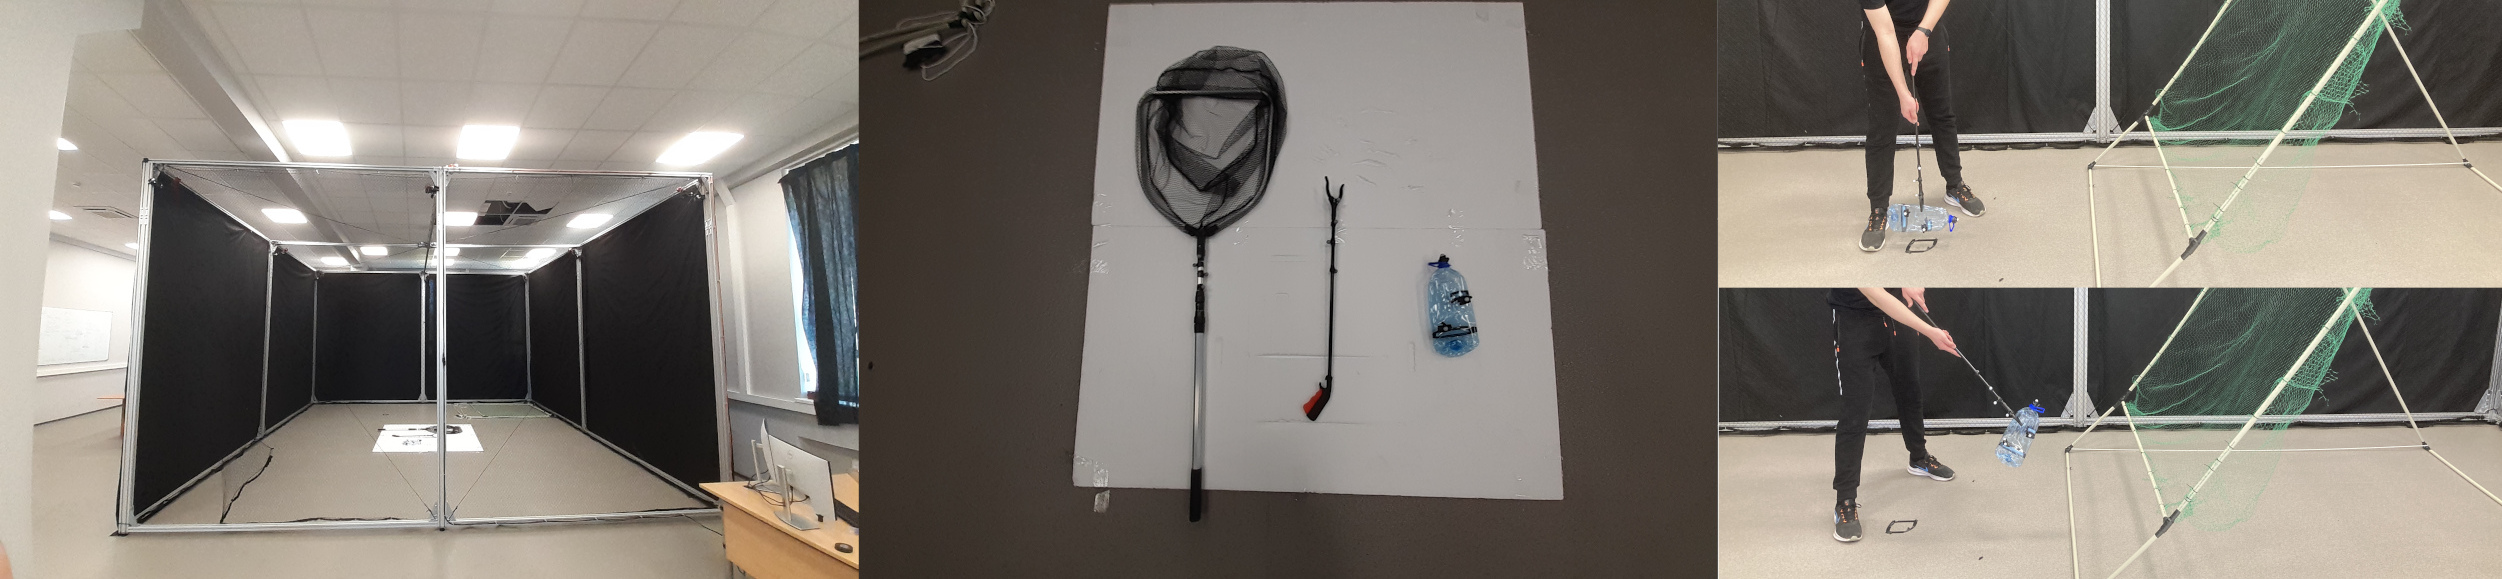
\includegraphics[width=16cm]{../img/mocap_process.jpg}}
	\caption{Motion capture equipment and process. \emph{(Photos by Peteris Racinskis)}}
	\label{fig:fig1}
\end{figure}

All demonstrations were recorded using \emph{OptiTrack} equipment that consists of a set of cameras, highly reflective markers to be attached to trackable objects and the \emph{Motive} software package which handles pose estimation and streaming. As shown in fig. \ref{fig:fig1}, a cage with 8 cameras installed serves to hide external sources of specular reflections from the cameras and confine moving objects such as drones from leaving the scene. To simulate an industrial robot end effector, a gripping hand tool was equipped with markers. Since the motivating application calls for throwing plastic bottles, one such was also marked to serve as basis for extrapolating target coordinates and identify the release point in a demonstration. A start point is laid down on the floor to serve as a datum for automatically separating the recorded demonstrations during pre-processing. Holding the effector stand-in here for at least a second before each demonstration provides a consistent signal that can be identified programmatically.

Nets were used to catch the thrown bottle and prevent damaging the markers. These were also marked to aid in delimiting the ballistic segment of the thrown object's flight. While in principle it is possible to detect an object in freefall by observing its acceleration, for the purposes of trajectory extrapolation this was deemed too prone to error~-- some impacts radically change the horizontal component of the object's velocity without breaking its fall, and the acceleration of the empty bottles proved to be affected by air resistance to a significant degree owing to their low terminal velocity.

In software, rigid body definitions were created for all object to be tracked. These were then streamed on the local network, relayed over \emph{Robot Operating System} (ROS) topics corresponding to each rigid body using a pre-existing package ROS and recorded into a bag file to be converted into a .csv data set. Over the course of this project, two data sets with roughly 150 and 50 demonstrations each were collected. The first was used in the development process but proved to contain throws beyond the capabilities of the robot hardware used. Therefore, a second data set of throws with less pronounced swings was produced to fit within the working volume of the robot arm.

\subsection{Pre-processing, extraction of implicit control signals}
\label{sec:preprocess}


\begin{figure}
	\centering
	\fbox{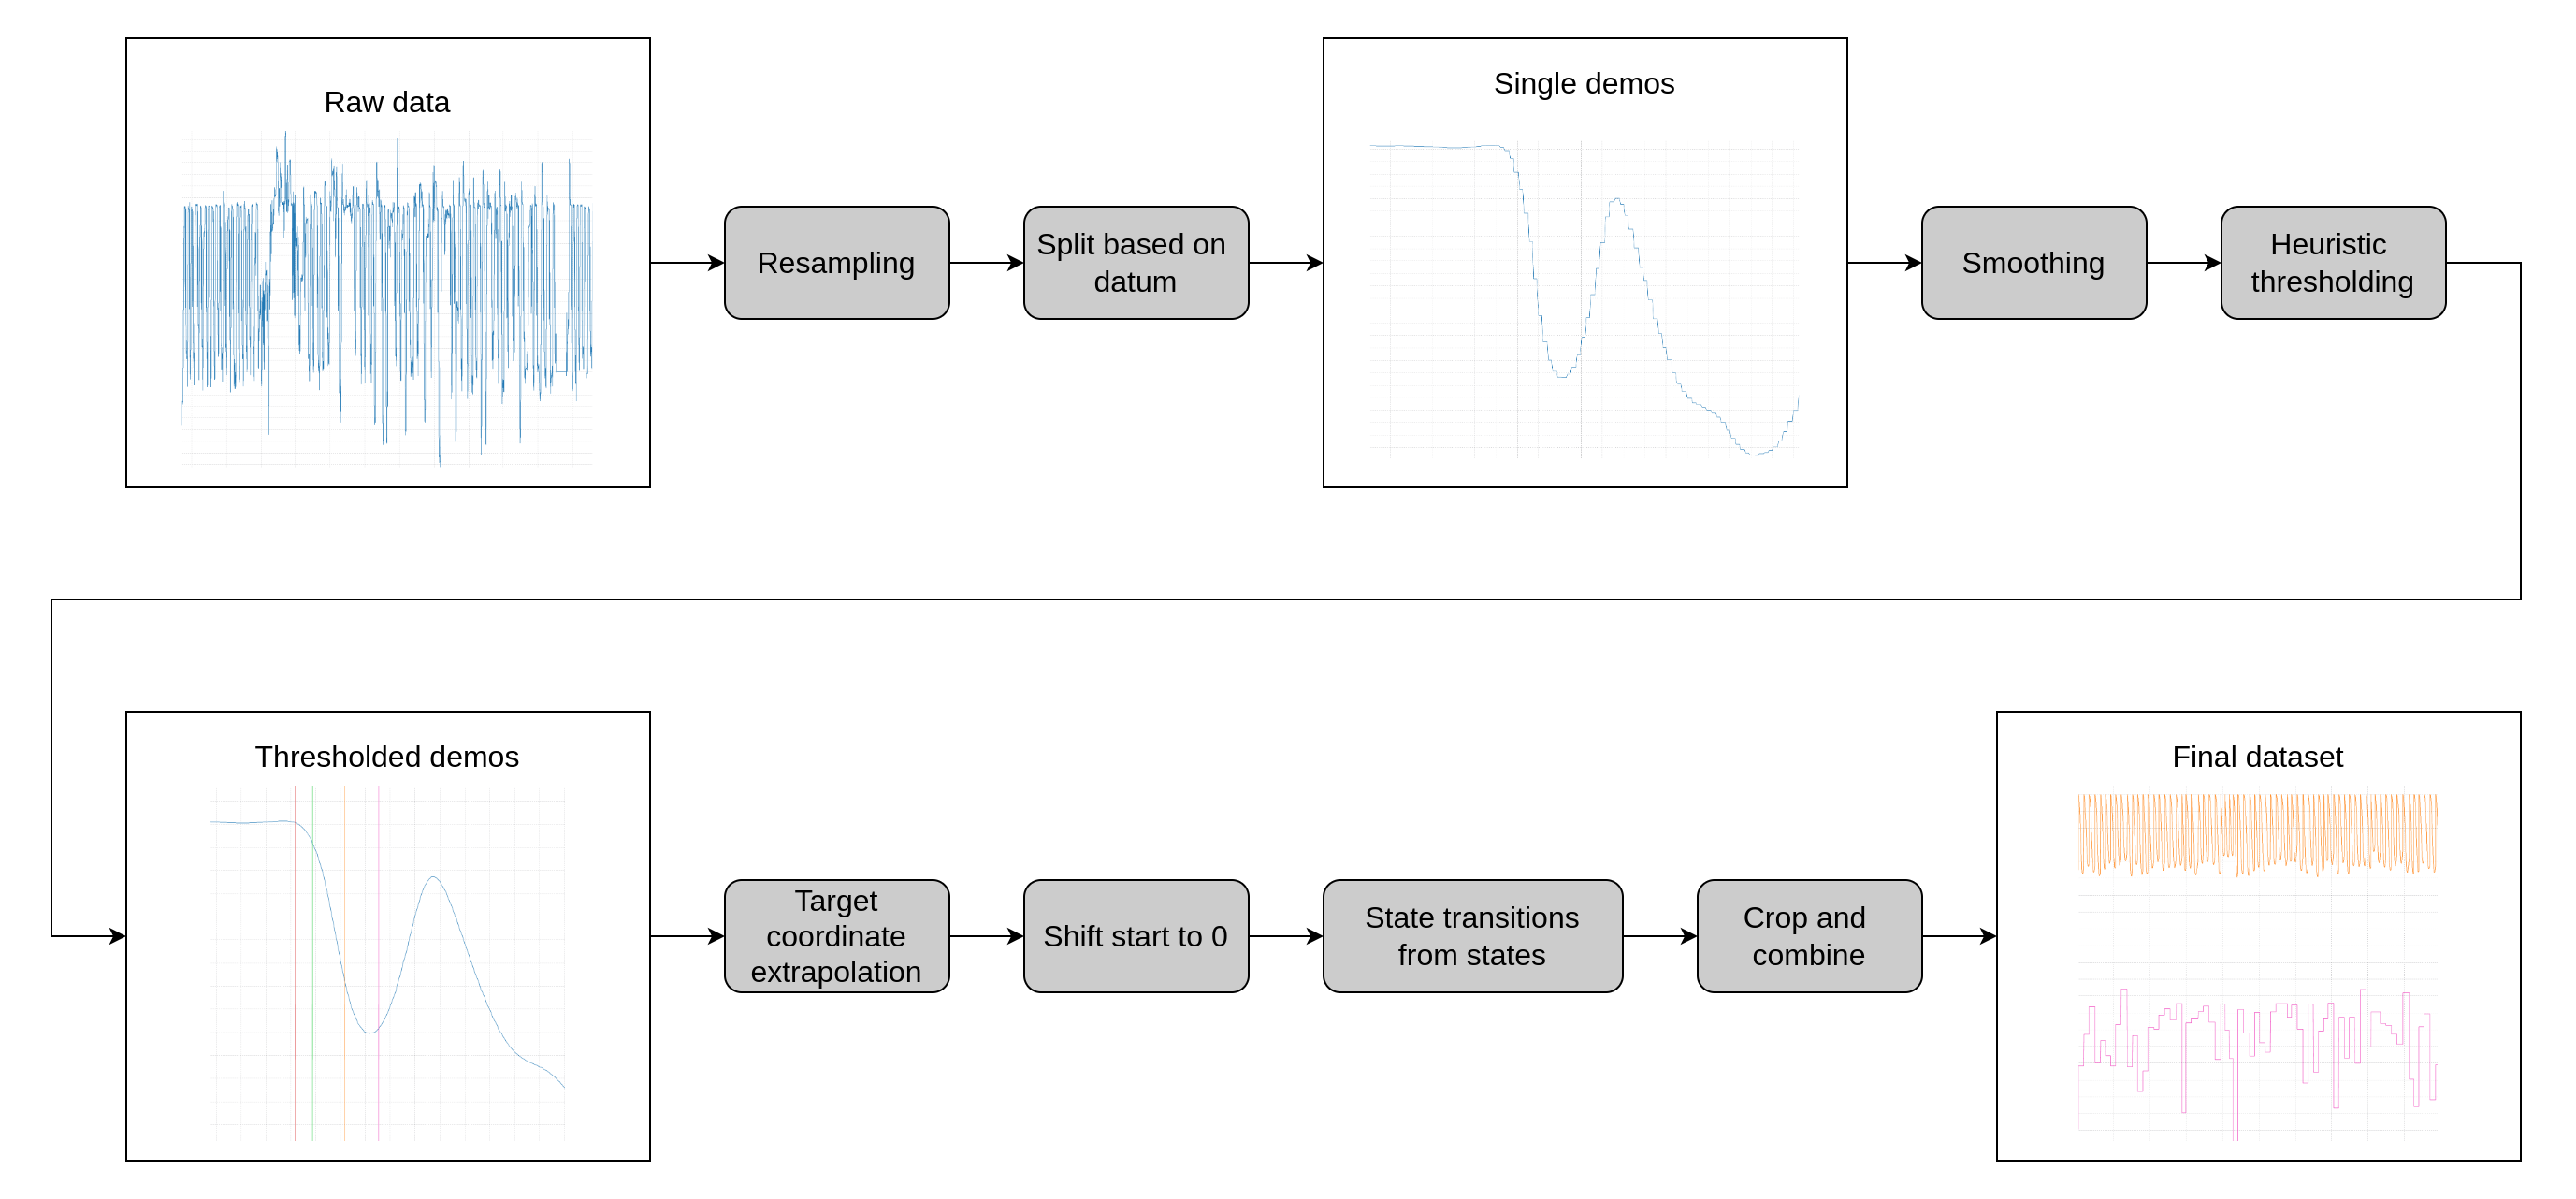
\includegraphics[width=16cm]{../img/preprocess_pipeline.png}}
	\caption{Pre-processing pipeline overview.}
	\label{fig:fig2}
\end{figure}

Figure \ref{fig:fig2} provides a schematic overview of the main steps involved in the data preparation process. For illustrative purposes, graphs of the effector x-coordinate with respect to time are used, but the final picture also contains the estimated target coordinate of each throw.

After each recording session, an entirely unstructured corpus is available. It contains timestamped pose observations collected at whatever intervals they happened to have been generated by the tracking software. Each observation only contains information about a single tracked body. A peculiarity of this particular recording method is that observations about each body tend to arrive in bursts:
\begin{equation}
    s^a_{t1}, s^a_{t2}, ..., s^b_{tm-1}, s^b_{tm}
\end{equation}
where $s^a_{t \in \mathbb{R}}$ corresponds to the observed state of object $a$ at time $t$.
Thus, to obtain sequential data in discrete time, it is necessary to resample the positions and orientations of all relevant bodies at a constant time step:
\begin{equation}
    (s^a_{1}, s^b_{1}, s^c_{1}), ..., (s^a_{k}, s^b_{k}, s^c_{k}) = s_1, ..., s_k
\end{equation}

A sampling frequency of $100Hz$ was selected to obtain spatial precision on the order of centimeters given the velocities involved. Fortuitously, the intervals between observed bursts in the actual data are generally on this order as well. Resampling is accomplished using forward fill interpolation, which introduces a slight sawtooth oscillation, but this is removed in the subsequent smoothing step along with other discontinuities.

After resampling, individual demonstrations are separated using the aforementioned consistent starting position. This may vary from recording session to recording session, so it needs to be identified and configured manually. Specifically, the condition used to identify demonstration start points is as follows:
\begin{align}
	t_{start} \in [t]^k_1: t < t_{start} \land (t_{start} - t < \Delta t_{max}) \Rightarrow \nonumber \\
	\Rightarrow x_t \in (x_{0} - \delta x, x_{0} + \delta x ), y_t \in  (y_{0} - \delta y, y_{0} + \delta y )
\end{align}

Which is to say that every observation no more than $\Delta t$ steps before $t_{start}$ has to lie within $\pm \delta x, \pm \delta y$ of the datum $(x_0, y_0)$. Each demonstration then consists of observations 

\begin{equation}
	(s_{t_{start}}, ... , s_{t_{start}+steps}), steps \in \mathbb{N}
\end{equation}
	
The constants $\Delta t, \delta x, \delta y, steps$ are determined experimentally to produce consistent observations for the particular task and may require tuning if the manner in which demonstrations are recorded changes. The newly split demonstrations are saved in separate files, thus allowing demonstrations generated in different sessions to be processed at once.

As further thresholding steps rely on estimates of pose derivatives, a smoothing step is first employed to remove noise and the slight sawtooth oscillation induced by the resampling step. This is accomplished by applying a rolling average kernel to the trajectory. Nevertheless, it was found that any estimate of derivatives would exacerbate what noise there was in the dataset, leading to inconsistent results. So a simplified estimator $\overline{x'_t}$, combining a correlate of the derivative $x'_t$ with a rolling average filter, was used with satisfactory results:
\begin{equation}
    x'_t \propto \overline{x'_t} = \sum_{i=t}^{t+m}  x_i - \sum_{i=t-m}^{t}  x_i
\end{equation}


\begin{figure}
	\centering
	\fbox{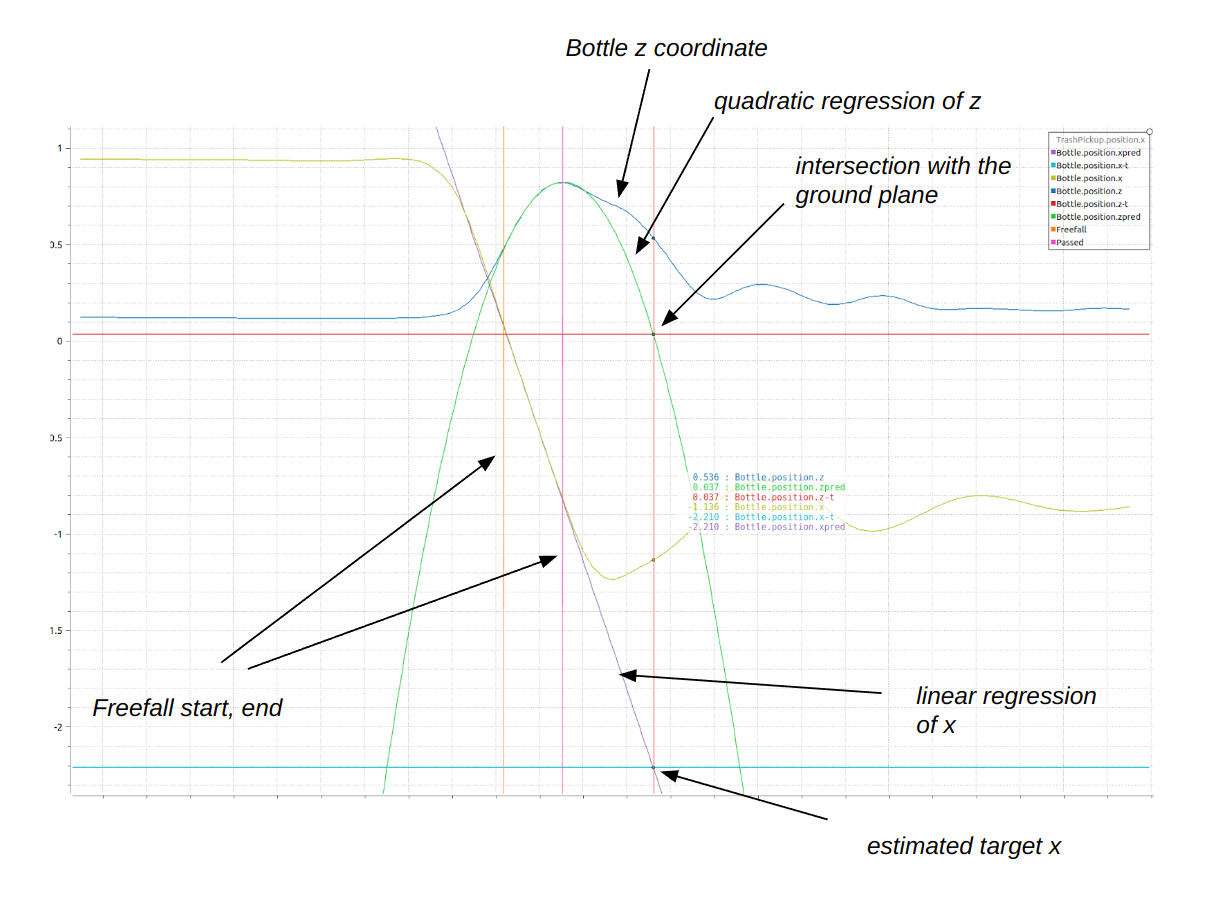
\includegraphics[width=11.6cm]{../img/target_regression.jpg}}
	\caption{Estimation of the throw target coordinates.}
	\label{fig:fig3}
\end{figure}


This was then used to compute threshold functions corresponding with the start of motion, actuator release and unfettered freefall of the bottle:

\begin{equation}
    f_{moving} (t) = \begin{cases}
        0 \text{ if } \forall u < t,  \lVert \overline{\left [  \boldsymbol{r}_{Effector}(u) \right ]'_u} \rVert  < \overline{v}_{moving} \\
        1 \text{ otherwise }
    \end{cases}
\end{equation}

\begin{equation}
    f_{release} (t) = \begin{cases}
        0 \text{ if } \forall u < t, \overline{ \left [ \lVert  \boldsymbol{r}_{Bottle}(u) -  \boldsymbol{r}_{Effector}(u)  \rVert \right ] ''_u} < \overline{a}_{release} \\
        1 \text{ otherwise }
    \end{cases}
\end{equation}

\begin{equation}
    f_{freefall} (t) = \begin{cases}
        0 \text{ if } \forall u < t,  \overline{ \left [ \lVert  \boldsymbol{r}_{Bottle}(u) -  \boldsymbol{r}_{Effector}(u)  \rVert \right ] '_u} < \overline{v}_{freefall} \\
        1 \text{ otherwise }
    \end{cases}
\end{equation}
where $\boldsymbol{r}$ corresponds to the position component of the observation vector. Note that in the first case, the norm of a vector derivative is used, whereas in the subsequent two it is the scalar derivative of a vector norm. As discussed in \ref{sec:collection}, the other terminating condition for the freefall segment of the bottle's trajectory is determined using the position of the net:
\begin{equation}
    f_{passed} (t) = \begin{cases}
        0 \text{ if } \forall u < t, x_{Bottle}(u) \geq x_{Net}(u) \\
        1 \text{ otherwise }
    \end{cases}
\end{equation}

The particular contents of the thresholding functions used are application-specific, but the method of detecting discrete events based on relative and absolute derivatives should prove broadly applicable. As with the split step, constants for thresholding were determined by way of inspection and would certainly be unique to each type of task. The output of $f_{release}$ serves as the gripper actuator signal estimate. $f_{moving}$ is used in the final align, crop and combine steps to determine the first observation to include in the dataset. $f_{freefall}, f_{passed}$ are used in estimating the desired target coordinates of each throw to give models the capability to be aimed. This is done by applying quadratic regression to the z-coordinate of the object thrown, finding its intersection with the ground plane in corresponding x and y-coordinates. The actuator signal and target coordinates are concatenated to each observation vector, with target coordinates being constant within each demonstration. A time signal is also added to each observation as this was found to improve the performance of feedforward models. Finally, when combining the demonstrations into a training data set, all position vectors are shifted so that the start of motion corresponds to the origin of the coordinate system. This way the models are trained to operate relative to the effector starting position.

\subsection{Models}
\label{sec:models}

We studied two classes of parametric models as part of this project -- simple feedforward neural networks and RNNs, operating autoregressively. The choice was motivated by two factors:
\begin{itemize}
	\item the dynamics of the problem were deemed to be simple enough that even small models would be able to model them adequately -- making it possible to quickly train on development machines with low parameter counts, using pre-existing code libraries;
	\item given the recent advances in employing sequence-to-sequence models for imitation learning tasks, it was decided that models with broadly similar footprints and characteristics should be used to enable further research in this direction.
\end{itemize}

After an initial hyperparameter discovery process, the values in table \ref{tab:table1} were arrived at for both model types respectively. A range of model sizes and training epoch counts was compared for both models. In the case of the recurrent neural network, performance with different learning rates was also evaluated. As the feedforward models were developed first, performance with and without a time signal in the input data was also compared. For the RNN architecture, GRU was selected as prior research suggests that it outperforms LSTM when dealing with small data sets of long sequences \citep{yang2020lstm}.

\begin{table}
	\caption{Model hyperparameters}
	\centering
	\begin{tabular}{lll}
		\toprule
		Parameter & Feedforward & RNN \\
		\midrule
		Architecture & 2 fully-connected hidden layers, ReLU  & GRU, fully connected linear output   \\
		Parameter counts     & 128-1024 perceptrons per layer & 128-512 perceptrons \\
		Training epochs     & 20-100       & 300-1200  \\
		Batch size    & 64       & 32  \\
		Optimizer    & \multicolumn{2}{c}{Adam}  \\
		Learning rate    & $10^{-4}$       & $10^{-3}, 10^{-4}$   \\
		\bottomrule
	\end{tabular}
	\label{tab:table1}
\end{table}

The basic model footprint is given as follows:

\begin{equation}
	(\boldsymbol{r}_{t+1}, \boldsymbol{q}_{t+1}, g_{t+1}) = \pi_{\theta}\left(\frac{t}{f_{sample}}, \boldsymbol{r}_{t}, \boldsymbol{q}_{t}, g_{t}, \boldsymbol{r}^{target}_t \right)
\end{equation}
where $\boldsymbol{r}_{t}, \boldsymbol{q}_{t}, g_{t}$ represent the end effector translation vector, orientation quaternion and gripper actuator signal respectively at time step $t$ in both the input and output. The input is augmented with a time/phase signal (discrete time step divided by the sampling frequency, in this case $100Hz$) relative to the start of the demonstration or generated trajectory, as well as the target coordinate vector $\boldsymbol{r}^{target}_t$ which corresponds to the extrapolated target coordinates in the demonstration data set and commanded throw coordinates at inference. The time signal was added to the input as it was found that trajectories generated by feedforward networks were liable to diverge without it, and the data sets thus modified were used for all training thereafter. The gripper control signal has values $\lbrace 0,1 \rbrace$ in the training data set.

For training both types of networks, state transitions $\left(\left(t,s_t,r^{target}_t\right), s_{t+1}\right)$ are constructed. In the case of the feedforward network, these state transitions are then shuffled and batched independently. For the RNN, pairs of feature-label sequences are formed corresponding to complete demonstrations, and the loss function is computed on the entire predicted output sequence. To hold these variable length sequences, a ragged tensor is used, which is batched along its first axis and ragged along the second. With both types of networks, the Huber loss function is utilized.


\subsection{Visualization and execution}
\label{sec:exec}

As discussed in the introduction, an important part of the reason for selecting throwing as our motivating application was the fact that it is easy for humans to judge the qualitative performance aspects of this task. To accomplish this, a means of visualizing the model outputs was required. When operating in open-loop mode (without interfacing with the physical or simulated environment -- running the model on its own previous outputs) it is possible to precompute trajectories and simply save them as sequences of robot states. To aid in estimating whether these trajectories were feasible, a tool for visualizing these sequences in the robot coordinate system was developed (fig. \ref{fig:vis_exec}, left).

Given a policy that synchronously predicts the state of the system at the next time step, there are multiple possible ways to use it in robot control. The simplest approach is static trajectory planning -- precompute a sequence of states and plan the motion between them. This is somewhat hindered by the lack of existing tools for precise time-parametrized Cartesian path planning in the ROS ecosystem. An alternative is a real-time pose following servo controller. The advantage of the latter approach is that closed-loop control is possible -- with state observations taken from the environment, potentially allowing the model to compensate for offsets in real time. However, this presents the challenge of tuning controller gains. The method that was ultimately employed was open-loop planning of Cartesian paths -- with timing approximated through a combination of time optimal trajectory generation \citep{kunz2012time}, followed by scaling the trajectory to the correct total duration. To control the gripper, a threshold value was set, the point in the trajectory at which this value was crossed was found, the corresponding joint state was computed, and a callback function was set up to trigger when this joint state was reached within some tolerance.

\begin{figure}
	\centering
	\fbox{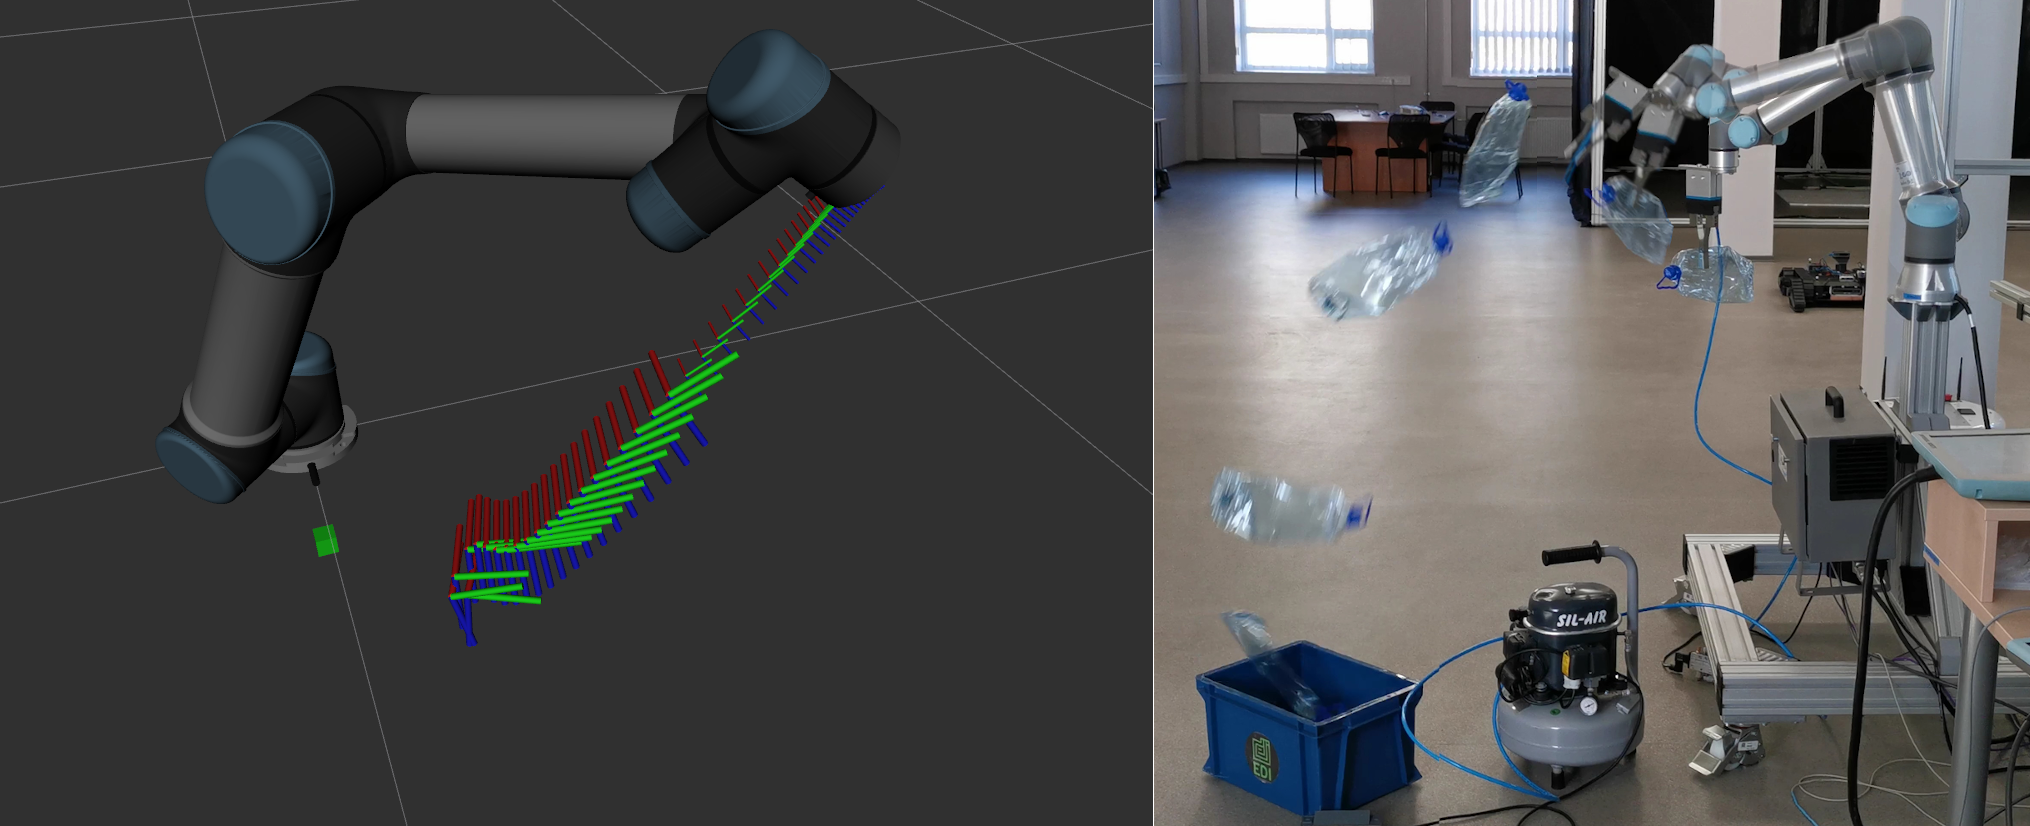
\includegraphics[width=16cm]{../img/vis_exec.png}}
	\caption{Visualization of pre-computed trajectories; execution of a throw on a real Ur5e robot.}
	\label{fig:vis_exec}
\end{figure}

While this is adequate for evaluating the positioning of the generated trajectories, and approximates the velocity profile closely enough for successful throws to be executed (fig.~\ref{fig:vis_exec}, right), a fully-featured time-parametrized Cartesian path planner or correctly tuned pose-following controller would be required to judge the throwing accuracy on real hardware and generalize our approach to other tasks. However, the development of such general purpose tools was deemed to be outside the scope of this project, the focus of which is on collection of demonstration data and imitation learning methods.

\subsection{Evaluation metrics}
\label{sec:eval}

To draw comparisons between models of different architectures, trained with differing hyperparameter sets, quantitative evaluation metrics need to be computed. As this is not a standard task with agreed-upon metrics and benchmarks, some 


\section{Results}

bla bla bla


\section{Discussion}

bla bla bla

\section{Conclusions}




\bibliographystyle{unsrtnat}
\bibliography{references}  %%% Uncomment this line and comment out the ``thebibliography'' section below to use the external .bib file (using bibtex) .



\end{document}
